% !TEX TS-program = pdflatex
\documentclass[11pt]{article}

% -------------------- Packages --------------------
\usepackage[a4paper,margin=1in]{geometry}
\usepackage{amsmath,amssymb}
\usepackage[T1]{fontenc}
\usepackage{lmodern}
\usepackage{xcolor}
\usepackage{tcolorbox}
\tcbuselibrary{skins,breakable}
\usepackage{enumitem}
\usepackage{hyperref}
\usepackage{tikz}
\usetikzlibrary{calc,patterns}

\pagestyle{empty}

% -------------------- Dark Theme Colors --------------------
\definecolor{bg}{HTML}{000000}
\definecolor{pairbg}{HTML}{121212}
\definecolor{solbg}{HTML}{0A0A0A}
\definecolor{border}{HTML}{2A2A2A}
\definecolor{text}{HTML}{FFFFFF}
\definecolor{muted}{HTML}{C9CDD3}
\definecolor{gold}{HTML}{FFD700}
\definecolor{green}{HTML}{4ADE80}
\definecolor{cyan}{HTML}{38BDF8}

\pagecolor{bg}
\color{text}

\hypersetup{
  colorlinks=true,
  linkcolor=cyan,
  urlcolor=cyan
}

\setlength{\parindent}{0pt}
\setlength{\parskip}{10pt}

\setlist[itemize]{left=1.4em,itemsep=6pt,topsep=6pt}
\setlist[enumerate]{left=1.6em,itemsep=4pt,topsep=4pt}

% -------------------- tcolorbox Base --------------------
\tcbset{
  enhanced,
  breakable,
  arc=12pt,
  boxrule=0.8pt,
  left=16pt,right=16pt,top=12pt,bottom=12pt
}

\newtcolorbox{QAPair}[1]{%
  colback=pairbg,
  colbacklower=solbg,
  colframe=border,
  coltext=text,
  title=\textcolor{gold}{\bfseries #1},
  fonttitle=\bfseries,
  coltitle=text,
  segmentation style={draw=border, dashed, line width=0.6pt},
}

\newtcolorbox{QuickBox}{%
  colback=pairbg,
  colframe=cyan,
  coltext=text,
  fontupper=\color{text},
  borderline north={4pt}{0pt}{cyan},
  arc=14pt,
  boxrule=0.8pt
}

% Helper for step headings
\newcommand{\Step}[1]{\textcolor{muted}{\textbf{Step #1:}}}

% -------------------- TikZ Styles --------------------
\tikzset{
  ax/.style={->, line width=1.0pt, draw=muted},
  grid/.style={draw=border, line width=0.35pt},
  lineC/.style={draw=cyan, line width=1.2pt},
  pt/.style={circle, fill=green, inner sep=1.6pt},
  lab/.style={text=text, font=\small},
  note/.style={text=muted, font=\small}
}

% ============================================================
\begin{document}

\begin{center}
{\LARGE\bfseries \textcolor{gold}{Miscellaneous Exercise 8 --- Solutions}}\\[-2pt]
\end{center}

\begin{QuickBox}
{\color{cyan}\bfseries Quick formulas (very useful)}\par\medskip
\begin{itemize}
\item \textbf{Slope (two points):} If $P(x_1,y_1),Q(x_2,y_2)$ then $m=\dfrac{y_2-y_1}{x_2-x_1}$.
\item \textbf{Angle between two lines:} $\tan\theta=\left|\dfrac{m_2-m_1}{1+m_1m_2}\right|$.
\item \textbf{Perpendicular lines:} $m_1m_2=-1$. \qquad \textbf{Parallel lines:} $m_1=m_2$.
\item \textbf{Distance:} $PQ=\sqrt{(x_2-x_1)^2+(y_2-y_1)^2}$.
\item \textbf{Midpoint:} $M=\left(\dfrac{x_1+x_2}{2},\dfrac{y_1+y_2}{2}\right)$.
\item \textbf{Slope-intercept:} $y=mx+c$. \quad \textbf{Intercept form:} $\dfrac{x}{a}+\dfrac{y}{b}=1$.
\item \textbf{Normal form:} $x\cos\alpha+y\sin\alpha=p$.
\end{itemize}
\end{QuickBox}

% ============================================================
% Q1 (MCQs)
\begin{QAPair}{Question 1 (i) --- MCQ}
\textcolor{gold}{\bfseries Question:} Slopes of two lines are $0$ and $\infty$. What is the angle between both lines?\par
\begin{itemize}
\item[(a)] $0^\circ$ \quad
\item[(b)] $60^\circ$ \quad
\item[(c)] $90^\circ$ \quad
\item[(d)] $180^\circ$
\end{itemize}
\tcblower
\textcolor{green}{\bfseries Answer:} \textbf{(c)}\par
\[
\begin{aligned}
\Step{1}\;& m=0 \Rightarrow \text{horizontal line (parallel to x-axis).}\\
\Step{2}\;& m=\infty \Rightarrow \text{vertical line (parallel to y-axis).}\\
\Step{3}\;& \text{Horizontal and vertical lines are perpendicular } \Rightarrow 90^\circ.
\end{aligned}
\]
\end{QAPair}

\begin{QAPair}{Question 1 (ii) --- MCQ}
\textcolor{gold}{\bfseries Question:} One angle of right triangle $ABC$ is determined by the line joining $A(1,2)$ and $B(2,3)$. Find the third angle.\par
\begin{itemize}
\item[(a)] $30^\circ$ \quad
\item[(b)] $45^\circ$ \quad
\item[(c)] $60^\circ$ \quad
\item[(d)] $80^\circ$
\end{itemize}
\tcblower
\textcolor{green}{\bfseries Answer:} \textbf{(b)}\par
\[
\begin{aligned}
\Step{1}\;& m_{AB}=\frac{3-2}{2-1}=1.\\
\Step{2}\;& \tan\theta = 1 \Rightarrow \theta=45^\circ \quad (\text{angle the line makes with x-axis}).\\
\Step{3}\;& \text{In a right triangle, angles sum }180^\circ\text{ and one angle is }90^\circ.\\
&\Rightarrow \text{third angle }=180^\circ-(90^\circ+45^\circ)=45^\circ.
\end{aligned}
\]
\end{QAPair}

\begin{QAPair}{Question 1 (iii) --- MCQ}
\textcolor{gold}{\bfseries Question:} Slope of points $(-1,6)$ and $(1,y)$ is $3$. What is $y$?\par
\begin{itemize}
\item[(a)] $10$ \quad
\item[(b)] $11$ \quad
\item[(c)] $-12$ \quad
\item[(d)] $12$
\end{itemize}
\tcblower
\textcolor{green}{\bfseries Answer:} \textbf{(d)}\par
\[
\begin{aligned}
\Step{1}\;& m=\frac{y-6}{1-(-1)}=\frac{y-6}{2}.\\
\Step{2}\;& \frac{y-6}{2}=3 \Rightarrow y-6=6 \Rightarrow y=12.
\end{aligned}
\]
\end{QAPair}

\begin{QAPair}{Question 1 (iv) --- MCQ}
\textcolor{gold}{\bfseries Question:} The line $5x-ky-3=0$ passes through $(1,2)$. What is $k$?\par
\begin{itemize}
\item[(a)] $1$ \quad
\item[(b)] $-1$ \quad
\item[(c)] $-2$ \quad
\item[(d)] $2$
\end{itemize}
\tcblower
\textcolor{green}{\bfseries Answer:} \textbf{(a)}\par
\[
\begin{aligned}
\Step{1}\;& 5(1)-k(2)-3=0\\
\Step{2}\;& 5-2k-3=0 \Rightarrow 2-2k=0 \Rightarrow k=1.
\end{aligned}
\]
\end{QAPair}

\begin{QAPair}{Question 1 (v) --- MCQ}
\textcolor{gold}{\bfseries Question:} The line $5x-6=0$ represents a line:\par
\begin{itemize}
\item[(a)] parallel to x-axis
\item[(b)] parallel to y-axis
\item[(c)] passing through origin
\item[(d)] touching both axes
\end{itemize}
\tcblower
\textcolor{green}{\bfseries Answer:} \textbf{(b)}\par
\[
\begin{aligned}
\Step{1}\;& 5x-6=0 \Rightarrow x=\frac{6}{5}.\\
\Step{2}\;& x=\text{constant is a vertical line} \Rightarrow \text{parallel to y-axis}.
\end{aligned}
\]
\end{QAPair}

\begin{QAPair}{Question 1 (vi) --- MCQ}
\textcolor{gold}{\bfseries Question:} Line $y=0$ represents:\par
\begin{itemize}
\item[(a)] x-axis \quad
\item[(b)] y-axis \quad
\item[(c)] a plane \quad
\item[(d)] a point
\end{itemize}
\tcblower
\textcolor{green}{\bfseries Answer:} \textbf{(a)}\par
\[
\Step{1}\; y=0 \text{ means all points have zero y-coordinate } \Rightarrow \text{x-axis.}
\]
\end{QAPair}

\begin{QAPair}{Question 1 (vii) --- MCQ}
\textcolor{gold}{\bfseries Question:} The line $y=b$ is above the x-axis, if\par
\begin{itemize}
\item[(a)] $b=0$ \quad
\item[(b)] $b<0$ \quad
\item[(c)] $b>0$ \quad
\item[(d)] $b\neq 0$
\end{itemize}
\tcblower
\textcolor{green}{\bfseries Answer:} \textbf{(c)}\par
\[
\Step{1}\; y=b \text{ is a horizontal line. Above x-axis means } b>0.
\]
\end{QAPair}

\begin{QAPair}{Question 1 (viii) --- MCQ}
\textcolor{gold}{\bfseries Question:} The line $x=a$ is left to the y-axis, if\par
\begin{itemize}
\item[(a)] $a=0$ \quad
\item[(b)] $a\neq 0$ \quad
\item[(c)] $a>0$ \quad
\item[(d)] $a<0$
\end{itemize}
\tcblower
\textcolor{green}{\bfseries Answer:} \textbf{(d)}\par
\[
\Step{1}\; x=a \text{ is vertical. Left of y-axis means } a<0.
\]
\end{QAPair}

\begin{QAPair}{Question 1 (ix) --- MCQ}
\textcolor{gold}{\bfseries Question:} Slope of a line $l$ is $-4$. What is slope of a line perpendicular to $l$?\par
\begin{itemize}
\item[(a)] $\dfrac14$ \quad
\item[(b)] $-\dfrac14$ \quad
\item[(c)] $4$ \quad
\item[(d)] $-4$
\end{itemize}
\tcblower
\textcolor{green}{\bfseries Answer:} \textbf{(a)}\par
\[
\begin{aligned}
\Step{1}\;& m_\perp=-\frac{1}{m}=-\frac{1}{-4}=\frac{1}{4}.
\end{aligned}
\]
\end{QAPair}

\begin{QAPair}{Question 1 (x) --- MCQ}
\textcolor{gold}{\bfseries Question:} Which of the following line has slope $\dfrac{2}{3}$?\par
\begin{itemize}
\item[(a)] $2x+3y=0$
\item[(b)] $2x-3y=2$
\item[(c)] $3x-2y=1$
\item[(d)] $3x+2y=3$
\end{itemize}
\tcblower
\textcolor{green}{\bfseries Answer:} \textbf{(b)}\par
\[
\begin{aligned}
\Step{1}\;& 2x-3y=2 \Rightarrow -3y=2-2x \Rightarrow y=\frac{2}{3}x-\frac{2}{3}.\\
\Step{2}\;& \Rightarrow \text{slope } m=\frac{2}{3}.
\end{aligned}
\]
\end{QAPair}

\begin{QAPair}{Question 1 (xi) --- MCQ}
\textcolor{gold}{\bfseries Question:} The line $y=5x-3$ is written in the form:\par
\begin{itemize}
\item[(a)] point-slope
\textcolor{text}{\quad}
\item[(b)] two-intercept
\textcolor{text}{\quad}
\item[(c)] slope-intercept
\textcolor{text}{\quad}
\item[(d)] two-point
\end{itemize}
\tcblower
\textcolor{green}{\bfseries Answer:} \textbf{(c)}\par
\[
\Step{1}\; y=mx+c \text{ is slope-intercept form. Here } m=5,\ c=-3.
\]
\end{QAPair}

\begin{QAPair}{Question 1 (xii) --- MCQ}
\textcolor{gold}{\bfseries Question:} x-intercept of the line $x+y=5$ is:\par
\begin{itemize}
\item[(a)] $1$ \quad
\item[(b)] $-1$ \quad
\item[(c)] $5$ \quad
\item[(d)] $-5$
\end{itemize}
\tcblower
\textcolor{green}{\bfseries Answer:} \textbf{(c)}\par
\[
\begin{aligned}
\Step{1}\;& \text{x-intercept: set } y=0.\\
\Step{2}\;& x+0=5 \Rightarrow x=5.
\end{aligned}
\]
\end{QAPair}

\begin{QAPair}{Question 1 (xiii) --- MCQ}
\textcolor{gold}{\bfseries Question:} A line intersects both axes at $(2,0)$ and $(0,7)$ respectively. Its y-intercept is:\par
\begin{itemize}
\item[(a)] $-2$ \quad
\item[(b)] $2$ \quad
\item[(c)] $-7$ \quad
\item[(d)] $7$
\end{itemize}
\tcblower
\textcolor{green}{\bfseries Answer:} \textbf{(d)}\par
\[
\Step{1}\; \text{y-intercept is the y-value when } x=0,\ \text{given point }(0,7)\Rightarrow 7.
\]
\end{QAPair}

\begin{QAPair}{Question 1 (xiv) --- MCQ}
\textcolor{gold}{\bfseries Question:} Point of intersection of lines $9x-7y=0$ and $8x-11y=0$ is:\par
\begin{itemize}
\item[(a)] $(0,0)$ \quad
\item[(b)] $(0,7)$ \quad
\item[(c)] $(9,0)$ \quad
\item[(d)] $(7,9)$
\end{itemize}
\tcblower
\textcolor{green}{\bfseries Answer:} \textbf{(a)}\par
\[
\begin{aligned}
\Step{1}\;& 9x-7y=0 \text{ passes through }(0,0).\\
\Step{2}\;& 8x-11y=0 \text{ also passes through }(0,0).\\
\Step{3}\;& \text{Since slopes are different, their only common point is }(0,0).
\end{aligned}
\]
\end{QAPair}

% ============================================================
% Q2
\begin{QAPair}{Question 2}
\textcolor{gold}{\bfseries Question:} Prove that $A(3,-10)$, $B(1,4)$ and $C(2,-3)$ are collinear points.\par
\tcblower
\textcolor{green}{\bfseries Answer:}
\[
\begin{aligned}
\Step{1}\;& m_{AB}=\frac{4-(-10)}{1-3}=\frac{14}{-2}=-7.\\
\Step{2}\;& m_{BC}=\frac{-3-4}{2-1}=\frac{-7}{1}=-7.\\
\Step{3}\;& m_{AB}=m_{BC}\ \Rightarrow\ A,B,C \text{ lie on the same straight line (collinear).}
\end{aligned}
\]
\end{QAPair}

% ============================================================
% Q3
\begin{QAPair}{Question 3}
\textcolor{gold}{\bfseries Question:} x-intercept of a line is double of y-intercept. Find the equation of line if it passes through $(2,1)$.\par
\tcblower
\textcolor{green}{\bfseries Answer:}
Let x-intercept $=a$ and y-intercept $=b$. Given $a=2b$.

\[
\begin{aligned}
\Step{1}\;& \text{Intercept form: }\frac{x}{a}+\frac{y}{b}=1.\\
\Step{2}\;& a=2b \Rightarrow \frac{x}{2b}+\frac{y}{b}=1.\\
\Step{3}\;& \text{Multiply by }b:\ \frac{x}{2}+y=b.\\
\Step{4}\;& \text{Use point }(2,1):\ \frac{2}{2}+1=b \Rightarrow 1+1=2 \Rightarrow b=2.\\
\Step{5}\;& a=2b=4.\\
\Step{6}\;& \Rightarrow \frac{x}{4}+\frac{y}{2}=1 \ \Longleftrightarrow\ x+2y=4.
\end{aligned}
\]
\[
\boxed{x+2y=4}
\]
\end{QAPair}

% ============================================================
% Q4
\begin{QAPair}{Question 4}
\textcolor{gold}{\bfseries Question:} Reduce $5x-2y+1=0$ into slope-intercept form and two-intercept form.\par
\tcblower
\textcolor{green}{\bfseries Answer:}

\textcolor{muted}{\bfseries (a) Slope-intercept form}\par
\[
\begin{aligned}
\Step{1}\;& 5x-2y+1=0 \Rightarrow -2y=-5x-1.\\
\Step{2}\;& y=\frac{5}{2}x+\frac{1}{2}.
\end{aligned}
\]
\[
\boxed{y=\frac{5}{2}x+\frac{1}{2}}
\]

\textcolor{muted}{\bfseries (b) Two-intercept form}\par
\[
\begin{aligned}
\Step{1}\;& \text{x-intercept: set }y=0 \Rightarrow 5x+1=0 \Rightarrow x=-\frac{1}{5}.\\
\Step{2}\;& \text{y-intercept: set }x=0 \Rightarrow -2y+1=0 \Rightarrow y=\frac{1}{2}.\\
\Step{3}\;& \Rightarrow \frac{x}{-\frac{1}{5}}+\frac{y}{\frac{1}{2}}=1.
\end{aligned}
\]
\[
\boxed{\frac{x}{-\frac{1}{5}}+\frac{y}{\frac{1}{2}}=1}
\]
\end{QAPair}

% ============================================================
% Q5
\begin{QAPair}{Question 5 (i)--(ii)}
\textcolor{gold}{\bfseries Question:} (i) Reduce $x-3y=3$ into intercept form and find x- and y-intercepts.\\
(ii) Find its slope and transform the equation into point-slope form.\par
\tcblower
\textcolor{green}{\bfseries Answer:}

\begin{enumerate}[label=\textbf{(\roman*)}]
\item \textbf{Intercepts and intercept form}
\[
\begin{aligned}
\Step{1}\;& \text{x-intercept: }y=0 \Rightarrow x=3 \Rightarrow (3,0).\\
\Step{2}\;& \text{y-intercept: }x=0 \Rightarrow -3y=3 \Rightarrow y=-1 \Rightarrow (0,-1).\\
\Step{3}\;& \text{Intercept form: }\frac{x}{3}+\frac{y}{-1}=1 \Rightarrow \frac{x}{3}-y=1.
\end{aligned}
\]
\[
\boxed{\frac{x}{3}-y=1}
\]

\item \textbf{Slope and point-slope form}
\[
\begin{aligned}
\Step{1}\;& x-3y=3 \Rightarrow -3y=3-x \Rightarrow y=\frac{1}{3}x-1.\\
\Step{2}\;& \text{Slope }m=\frac{1}{3}.\\
\Step{3}\;& \text{Using point }(3,0):\ y-0=\frac{1}{3}(x-3).
\end{aligned}
\]
\[
\boxed{y=\frac{1}{3}(x-3)}
\]
\end{enumerate}
\end{QAPair}

% ============================================================
% Q6
\begin{QAPair}{Question 6}
\textcolor{gold}{\bfseries Question:} Normal form of an equation of line is $x\cos150^\circ+y\sin150^\circ=10$.\\
Transform it into slope-intercept form and find its slope and y-intercept.\par
\tcblower
\textcolor{green}{\bfseries Answer:}
\[
\begin{aligned}
\Step{1}\;& \cos150^\circ=-\frac{\sqrt3}{2},\quad \sin150^\circ=\frac{1}{2}.\\
\Step{2}\;& x\left(-\frac{\sqrt3}{2}\right)+y\left(\frac12\right)=10.\\
\Step{3}\;& \text{Multiply by }2:\ -\sqrt3\,x+y=20.\\
\Step{4}\;& y=\sqrt3\,x+20.
\end{aligned}
\]
\[
\boxed{y=\sqrt3\,x+20},\qquad \boxed{m=\sqrt3},\qquad \boxed{\text{y-intercept}=20}.
\]
\end{QAPair}

% ============================================================
% Q7
\begin{QAPair}{Question 7 (i)--(iii)}
\textcolor{gold}{\bfseries Question:} From the given graph of triangle $ABC$: \\
(i) Find vertices of triangle $ABC$.\\
(ii) Calculate slopes of its sides.\\
(iii) Find interior angles of the triangle.\par
\tcblower
\textcolor{green}{\bfseries Answer:}

\textcolor{muted}{(From the graph, by counting grid units)}\par
\[
\boxed{A(-4,3),\quad B(8,5),\quad C(1,9)}.
\]

\begin{enumerate}[label=\textbf{(\roman*)}]
\item \textbf{Vertices:} $A(-4,3)$, $B(8,5)$, $C(1,9)$.

\item \textbf{Slopes of sides}
\[
\begin{aligned}
m_{AB}&=\frac{5-3}{8-(-4)}=\frac{2}{12}=\frac{1}{6},\\[4pt]
m_{BC}&=\frac{9-5}{1-8}=\frac{4}{-7}=-\frac{4}{7},\\[4pt]
m_{CA}&=\frac{3-9}{-4-1}=\frac{-6}{-5}=\frac{6}{5}.
\end{aligned}
\]

\item \textbf{Interior angles (using dot product / cosine rule)}\par
Let
\[
\overrightarrow{AB}=(12,2),\quad \overrightarrow{AC}=(5,6),\quad
\overrightarrow{BA}=(-12,-2),\quad \overrightarrow{BC}=(-7,4).
\]
Then
\[
\angle A \approx 40.7^\circ,\qquad
\angle B \approx 39.2^\circ,\qquad
\angle C \approx 100.1^\circ.
\]
(\textcolor{muted}{They add to }$180^\circ$.)

\end{enumerate}

\textcolor{muted}{\bfseries Sketch (triangle on axes)}\par
\begin{center}
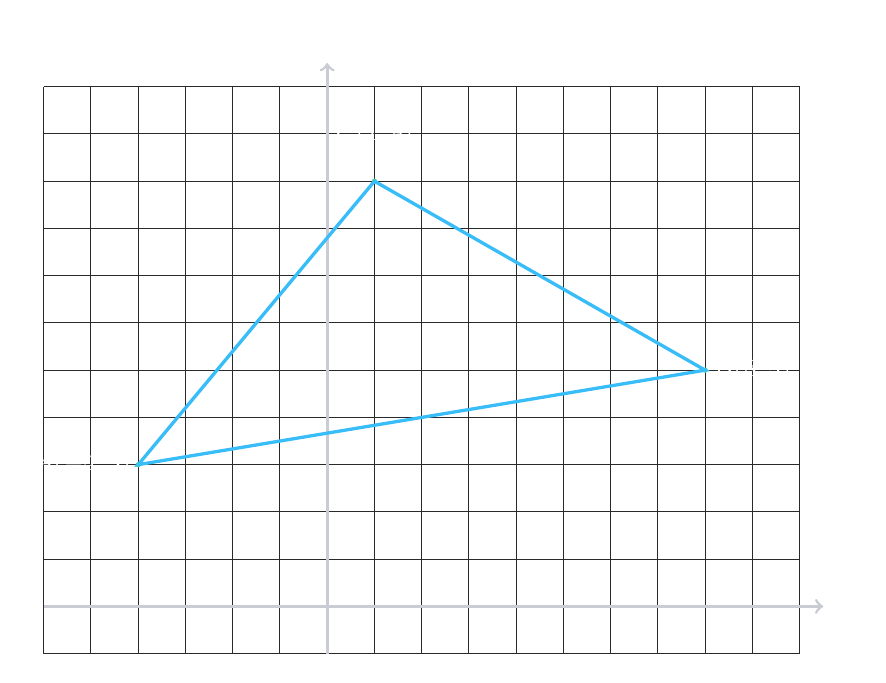
\begin{tikzpicture}[scale=0.6]
  % grid
  \draw[grid] (-6,-1) grid (10,11);
  % axes
  \draw[ax] (-6,0) -- (10.5,0) node[lab, right] {$x$};
  \draw[ax] (0,-1) -- (0,11.5) node[lab, above] {$y$};

  % points
  \fill[pt] (-4,3) circle (1.6pt) node[lab, left] {$A(-4,3)$};
  \fill[pt] (8,5) circle (1.6pt) node[lab, right] {$B(8,5)$};
  \fill[pt] (1,9) circle (1.6pt) node[lab, above] {$C(1,9)$};

  % sides
  \draw[lineC] (-4,3) -- (8,5) -- (1,9) -- cycle;
\end{tikzpicture}
\end{center}
\end{QAPair}

% ============================================================
% Q8
\begin{QAPair}{Question 8 (i)--(iv)}
\textcolor{gold}{\bfseries Question:} Two points $P(4,-1)$ and $Q(8,3)$ lie on a line. Find: \\
(i) midpoint $M$ of $PQ$ \quad
(ii) slope of $PM$ \quad
(iii) equation of line parallel to $PQ$ through $(-2,2)$ \quad
(iv) equation of line perpendicular to $PQ$ through $(-2,2)$.\par
\tcblower
\textcolor{green}{\bfseries Answer:}

\[
\begin{aligned}
\Step{1}\;& M=\left(\frac{4+8}{2},\frac{-1+3}{2}\right)=(6,1).\\[4pt]
\Step{2}\;& m_{PQ}=\frac{3-(-1)}{8-4}=\frac{4}{4}=1.\\
&\Rightarrow m_{PM}=1\quad(\text{same line}).\\[6pt]
\Step{3}\;& \text{Parallel through }(-2,2):\ y-2=1(x+2)\Rightarrow y=x+4.\\[4pt]
\Step{4}\;& \text{Perpendicular slope }=-1:\ y-2=-1(x+2)\Rightarrow y=-x.
\end{aligned}
\]
\[
\boxed{M(6,1)},\qquad \boxed{m_{PM}=1},\qquad \boxed{y=x+4},\qquad \boxed{y=-x}.
\]
\end{QAPair}

% ============================================================
% Q9
\begin{QAPair}{Question 9 (i)--(iv)}
\textcolor{gold}{\bfseries Question:} Two points $A(2,-2)$ and $B(4,6)$ lie on a line. Find: \\
(i) length of $AB$ \quad
(ii) slope of $BA$ \quad
(iii) values of $a$ and $b$ when the line $AB$ is $ax+by-10=0$ \quad
(iv) equation of line parallel to $AB$ passing through $(0,3)$.\par
\tcblower
\textcolor{green}{\bfseries Answer:}

\begin{enumerate}[label=\textbf{(\roman*)}]
\item \textbf{Length}
\[
AB=\sqrt{(4-2)^2+(6-(-2))^2}=\sqrt{2^2+8^2}=\sqrt{68}=2\sqrt{17}.
\]

\item \textbf{Slope}
\[
m_{BA}=\frac{-2-6}{2-4}=\frac{-8}{-2}=4.
\]

\item \textbf{Find $a,b$ in $ax+by-10=0$}\par
First find equation of $AB$:
\[
y+2=4(x-2)\Rightarrow y=4x-10 \Rightarrow 4x-y-10=0.
\]
Comparing with $ax+by-10=0$ gives:
\[
\boxed{a=4,\quad b=-1}.
\]

\item \textbf{Parallel through $(0,3)$ (same slope 4)}
\[
y-3=4(x-0)\Rightarrow \boxed{y=4x+3}.
\]
\end{enumerate}
\end{QAPair}

% ============================================================
% Q10
\begin{QAPair}{Question 10}
\textcolor{gold}{\bfseries Question:} Find equation of the line passing through midpoint of $(4,4)$ and $(8,0)$ and parallel to the line having slope $\dfrac{2}{5}$.\par
\tcblower
\textcolor{green}{\bfseries Answer:}
\[
\begin{aligned}
\Step{1}\;& \text{Midpoint }M=\left(\frac{4+8}{2},\frac{4+0}{2}\right)=(6,2).\\
\Step{2}\;& \text{Slope }m=\frac{2}{5}.\\
\Step{3}\;& y-2=\frac{2}{5}(x-6).\\
\Step{4}\;& 5y-10=2x-12 \Rightarrow 2x-5y-2=0.
\end{aligned}
\]
\[
\boxed{y-2=\frac{2}{5}(x-6)}\qquad\text{or}\qquad \boxed{2x-5y-2=0}.
\]
\end{QAPair}

% ============================================================
% Q11
\begin{QAPair}{Question 11 (i)--(iv)}
\textcolor{gold}{\bfseries Question:} Lines $OC$ and $AB$ are shown in the graph. Find: \\
(i) coordinates of end points of $OC$ and $AB$ \\
(ii) slopes of both lines \\
(iii) equations of both lines \\
(iv) coordinates of point of intersection of both lines.\par
\tcblower
\textcolor{green}{\bfseries Answer:}

\textcolor{muted}{(From the graph, by counting grid units)}\par
\[
\boxed{O(0,0),\ C(6,7),\ A(-3,5),\ B(6,2)}.
\]

\begin{enumerate}[label=\textbf{(\roman*)}]
\item \textbf{Endpoints:} $OC:\ O(0,0),C(6,7)$ and $AB:\ A(-3,5),B(6,2)$.

\item \textbf{Slopes}
\[
m_{OC}=\frac{7-0}{6-0}=\frac{7}{6},\qquad
m_{AB}=\frac{2-5}{6-(-3)}=\frac{-3}{9}=-\frac{1}{3}.
\]

\item \textbf{Equations}
\[
OC:\ y=\frac{7}{6}x.
\]
For $AB$ using point $A(-3,5)$:
\[
y-5=-\frac13(x+3)\Rightarrow y=4-\frac{x}{3}
\Rightarrow x+3y=12.
\]

\item \textbf{Intersection}
\[
\frac{7}{6}x=4-\frac{x}{3}
\Rightarrow \frac{7}{6}x=4-\frac{2}{6}x
\Rightarrow \frac{9}{6}x=4
\Rightarrow x=\frac{24}{9}=\frac{8}{3}.
\]
\[
y=\frac{7}{6}\cdot\frac{8}{3}=\frac{56}{18}=\frac{28}{9}.
\]
\[
\boxed{\text{Intersection}=\left(\frac{8}{3},\frac{28}{9}\right)}.
\]
\end{enumerate}

\textcolor{muted}{\bfseries Sketch (lines on axes)}\par
\begin{center}
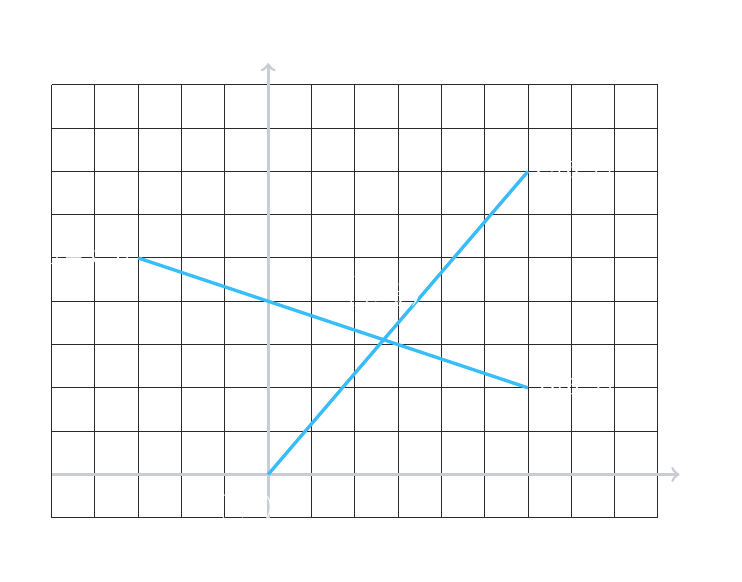
\begin{tikzpicture}[scale=0.55]
  \draw[grid] (-5,-1) grid (9,9);
  \draw[ax] (-5,0) -- (9.5,0) node[lab, right] {$x$};
  \draw[ax] (0,-1) -- (0,9.5) node[lab, above] {$y$};

  \fill[pt] (0,0) node[lab, below left] {$O(0,0)$};
  \fill[pt] (6,7) node[lab, right] {$C(6,7)$};
  \fill[pt] (-3,5) node[lab, left] {$A(-3,5)$};
  \fill[pt] (6,2) node[lab, right] {$B(6,2)$};

  \draw[lineC] (0,0) -- (6,7);
  \draw[lineC] (-3,5) -- (6,2);

  \fill[pt] (8/3,28/9) node[lab, above] {$\left(\frac{8}{3},\frac{28}{9}\right)$};
\end{tikzpicture}
\end{center}
\end{QAPair}

% ============================================================
% Q12
\begin{QAPair}{Question 12 (i)--(iv)}
\textcolor{gold}{\bfseries Question:} Locate two points on the coordinate plane that satisfy $x-2y=2$. Find: \\
(i) slope of segment $l$ connecting the two points \\
(ii) slope of segment $p$ perpendicular to $l$ \\
(iii) midpoint of segment $l$ \\
(iv) equation of line passing through midpoint of $l$ and slope of $p$.\par
\tcblower
\textcolor{green}{\bfseries Answer:}

Choose two easy points on $x-2y=2$:
\[
\text{If }y=0,\ x=2 \Rightarrow P(2,0);\qquad
\text{If }y=1,\ x=4 \Rightarrow Q(4,1).
\]

\begin{enumerate}[label=\textbf{(\roman*)}]
\item \textbf{Slope of $l=PQ$}
\[
m_l=\frac{1-0}{4-2}=\frac{1}{2}.
\]

\item \textbf{Slope of $p$ perpendicular to $l$}
\[
m_p=-\frac{1}{m_l}=-\frac{1}{\frac12}=-2.
\]

\item \textbf{Midpoint of $l$}
\[
M=\left(\frac{2+4}{2},\frac{0+1}{2}\right)=(3,\tfrac12).
\]

\item \textbf{Line through $M$ with slope $m_p=-2$}
\[
y-\frac12=-2(x-3)
\Rightarrow y=-2x+\frac{13}{2}.
\]
(Standard form: $4x+2y-13=0$.)
\end{enumerate}

\textcolor{muted}{\bfseries Sketch (two points and perpendicular-slope line)}\par
\begin{center}
\begin{tikzpicture}[scale=0.75]
  \draw[grid] (-1,-2) grid (7,5);
  \draw[ax] (-1,0) -- (7.5,0) node[lab, right] {$x$};
  \draw[ax] (0,-2) -- (0,5.5) node[lab, above] {$y$};

  \fill[pt] (2,0) node[lab, below] {$P(2,0)$};
  \fill[pt] (4,1) node[lab, right] {$Q(4,1)$};
  \fill[pt] (3,0.5) node[lab, above] {$M(3,\tfrac12)$};

  \draw[lineC] (2,0) -- (4,1) node[note, midway, above] {$l$};

  % line through M with slope -2: y = -2x + 13/2
  \draw[lineC] (-1, 13/2 -2*(-1)) -- (7, 13/2 -2*(7)) node[note, near end, right] {$p$};
\end{tikzpicture}
\end{center}
\end{QAPair}

\end{document}
